\documentclass[]{report}
\renewcommand\thesection{\arabic{section}}%for page numbering in arabics
\usepackage{graphicx,tabularx}%for figures and tables
\usepackage[utf8]{inputenc} %allows special characters such as ä, ö, ỳ
\usepackage[english]{babel}  %set the language to English
\usepackage[margin=1.5in]{geometry} %change page margins 
\usepackage{sectsty}%section headers

\setcounter{secnumdepth}{3}


\allsectionsfont{\sffamily\large}
\subsectionfont{\sffamily\normalsize}
\linespread{1.2}% line distance
\usepackage{lipsum}% http://ctan.org/pkg/lipsum
\usepackage{caption}%use for captions on tables
%use this exact command. The style and bibliographystyle has to be authoryear (Havard). The sorting is nyt: name, year, title so that the bibliography is sorted alphabetically. firstinits=true shortens the names: Albert Einstein -> A. Einstein
\usepackage[backend=biber,style=authoryear,bibstyle=authoryear,sorting=nyt,firstinits=true]{biblatex}
\setlength\parindent{0pt}%include this so that your paragraphs don't indent automatically
\addbibresource{ARDA-ML.bib} %this attaches your bib-file, your bibliography (must be in the same folder)
\usepackage[compact]{titlesec}%include title formatting package

% Title Page
\title{Exploring the Impact of Training Iterations on Object Detection Accuracy in Computer Vision}
\author{Louis Ferger Andrews and Paul Recker}
\date{December 18th 2023 \\Module: ARDA \\Venlo, Limburg, Netherlands}


\begin{document}
\maketitle

\begin{abstract}
This is the abstract.
\pagenumbering{roman}
\end{abstract}

\tableofcontents
\setcounter{page}{3}
%\listoffigures %UNCOMMENT IF YOU HAVE FIGURES
%\listoftables %UNCOMMENT IF YOU HAVE TABLES
\pagebreak
\pagenumbering{arabic}	
	


\section{Introduction}
The first chapter of the given investigation will provide the guiding research question that will be accompanied by background information based on the given topic. Expanding on this foundation, a hypothesis will be stated, that shall thereafter be tested during the conducted experiment, for the given investigation.  lalalalal

\subsection{Research Question}
How does the number of training iterations a machine learning algorithm is trained with affect the object detection accuracy of a computer vision program?

\subsection{Context and Background}
Computer vision, a rapidly growing field found in artificial intelligence, that enables computer systems to interpret visual data through the use of machine learning. It aims to replicate the human visual system, allowing it to identify objects found in images, pictures or live video feeds. The increased adoption of computer vision in various fields, such as medicine, automotive, education, security or agriculture, underlines its widespread utilization and adoption. This is primarily reasoned due to its significant impact on efficiency, effectiveness and the enhancement of various applications found in these fields. Hence its importance and impact on the future are continuously increasing. 

\subsubsection{Computer vision}
To comprehend how computer vision systems function, it is vital to comprehend the correlation they have with the human biological vision system. This is because computer vision systems follow the same principles as the human visual system. It is hypothesised by neurobiologists, that the brain aims to detect patterns it is familiar with to decode into objects. Hence the brain uses the eyes as sensors, capturing the surroundings to create a visual representation. The brain then analyses the representation for recognizable patterns, creating predictions about the objects present. The given familiar patterns are derived from previous encounters with similar objects(further explained in 1.2.2). Computer vision models aim to replicate this process, utilising the camera to create images of real-world properties. Following image processing, the data undergoes analysis to identify familiar patterns, allowing confident predictions about the objects depicted in the image, to be made \parencite{Hohman2020}.

\subsubsection{Machine learning }
Machine learning, within the field of artificial intelligence, is an approach that enables a program to utilise historical data to learn and train with, by recognising patterns in data. This allows the program to make future predictions by drawing upon the knowledge acquired during training with past historical data. Consequently, the program gains the ability to generate independent predictions without being explicitly programmed for specific predictions. This process replicates the biological approach of a child learning the names of new objects. When a child is confronted with an unfamiliar object, the child may attempt to predict what the object could be based on similarities with a known object, but won't be able to accurately identify the object. However,  if the child is given the name of the object and is exposed to multiple instances of the given object, the child will start learning and become more adept at recognizing and identifying the object when encountered again. Machine learning functions on the same basis. The more the program is trained, the more refined its predictions become, as it accumulates experiences in accurately predicting specific objects. This learning process, also referred to as machine learning training, enhances the program's ability to create accurate predictions over time. 

\subsubsection{Importance of accuracy in computer vision programs}
With the widespread integration of computer vision programs across various fields, the accuracy of the given models assumes a key significance. Tesla, an automotive market leader for self-driving cars, has widely adopted computer vision programs based on machine learning for their autonomous vehicles. It is crucial for the given programs to accurately identify objects with a high level of confidence in real-time, enabling it to create a picture of the environment it is operating in. Hence resulting in a close-to-perfect detection accuracy. The significance lies in the fact that a failure to identify an object, can result in real-world consequences such as a collision with a different object. Therefore accuracy is a pivotal aspect of computer vision programs for widespread acceptance. Furthermore recognising that a low accuracy will directly translate into high error rates in programs utilising computer vision and retrospectively resulting in potential catastrophic implications. Therefore it can be stated that the accuracy of computer vision programs based on machine learning plays a pivotal role in the practical implementation of such models in real-world applications. 


\subsection{Hypothesis}
Based on the context provided, it can be hypothesised that increasing the training iterations for the machine learning algorithm will have a direct correlation with the accuracy of the object detection model. Hence the greater the number of training iterations the program goes through, the greater the accuracy should become. This hypothesis is based on the fact that each additional iteration of training, will allow the model to converge towards a more optimised state by adjusting its parameters to minimize the differences between the training and the test data.\\


It is expected that during the initial training phases of the given experiment, specifically between 1,000 and 3,000 iterations, the model might face challenges in identifying objects in the test images accurately. In the cases where it does recognise the given objects, it is probable that it will do so with only a minimal degree of accuracy. This is thereafter expected to greatly change as the model rapidly begins to gain a basic understanding of the objects it is confronted with based on its training. Therefore it is appropriate to assume that during the stage, between  4,000 and 13,000 the greatest increase in accuracy should be displayed.  Beyond this point, it can be expected that as the model reaches a substantial accuracy of around 80\%, it can be hypothesised that the growth in accuracy will steadily decrease as the model converges towards an optimal state and the accuracy plateaus.\\


Furthermore, it can be theorised that a decrease in the model's loss should lead to an increase in accuracy, considering the inverse relationship between loss and accuracy, where a loss reduction indicates an improved performance as loss is measured by testing for accuracy.\\


In summary, a significant correlation between the accuracy and the number of training iterations for the machine learning algorithm is expected, which will gradually decrease as the model approaches its optimal state.


 
\section{Methods}
This chapter covers the methodology used to conduct the experiment which is the main focus of this paper.
It will cover the research design, the experiment setup and execution, as well as the data transformation 
and visualisation.\\

\subsection{Research Design}
The research of this paper is based on empirical and quantitative data collected from an experiment.
The experiment is made up of the following variables, the independent variable, the number of training iterations the
program is trained with, and the dependent variable, the accuracy of the model. To make sure results are accurate and consistent, 
all iterations will use the same machine learning algorithm,
the same dataset, the same evaluation data, and run on the same hardware.
The data which is being collected and analyzed is the number of iterations (categorical ordinal), the accuracy
and loss (continuous ratio), and the relation between them.\\

\begin{table}[h]
\centering
\begin{tabularx}{\textwidth}{|>{\hsize=.5\hsize}X|>{\hsize=1.5\hsize}X|}
\hline
\textbf{Type} & \textbf{Variable} \\
\hline
Independent Variable & 
\begin{tabular}{@{}l@{}}
\textbullet{} Number of Iterations  \\
\end{tabular} 
\\
\hline
Dependent Variable & 
\begin{tabular}{@{}l@{}}
\textbullet{} Accuracy of the Model\\
\end{tabular} 
\\
\hline
Controlled Variable & 
\begin{tabular}{@{}l@{}}
\textbullet{} Machine Learning Algorithm \\
\textbullet{} Dataset, Evaluation Data \\
\textbullet{} Hardware \\
\end{tabular} 
\\
\hline
\end{tabularx}
\caption{Key Variables of the Experiment}
\label{table:1}
\end{table}

\subsection{Experiment Setup and Execution}
The program "CreateML" from \cite{Apple} was used to carry out this experiment. It is a user-friendly and powerful 
tool that allows developers to create custom machine-learning models without the need for extensive expertise in the field.
CreateML simplified the process of creating and training an object detection model by providing a graphical user interface which 
just takes the input dataset and the desired parameters. The object detection model uses the YOLOv2 \parencite{Jaina} algorithm.
"You Only Look Once" (YOLO) is a state-of-the-art, real-time object detection algorithm introduced in 2015" \parencite{Keita2022}. 
The dataset used to train the object detection model is \citetitle{pascal2023} which is a collection of around 10000 images including classes
like persons, vehicles and animals. The experiment was run on a MacBook Air 2020 with an Apple M1 chip and 8GB of RAM. To ensure the 
result were unbaised the "Batch Size" was left on auto and the "Grid Size" was set to 13x13.\\

\newpage
Overall the model was trained 20.000 times and every 1000 iterations a snapshot of the model was taken and evaluated using
specific images. 
The classes and images chosen include: Boat, Dog, Person, Plant, Wheel (See Appendix~\ref{app:test-pictures}).
\begin{figure}[h]
  \centering
  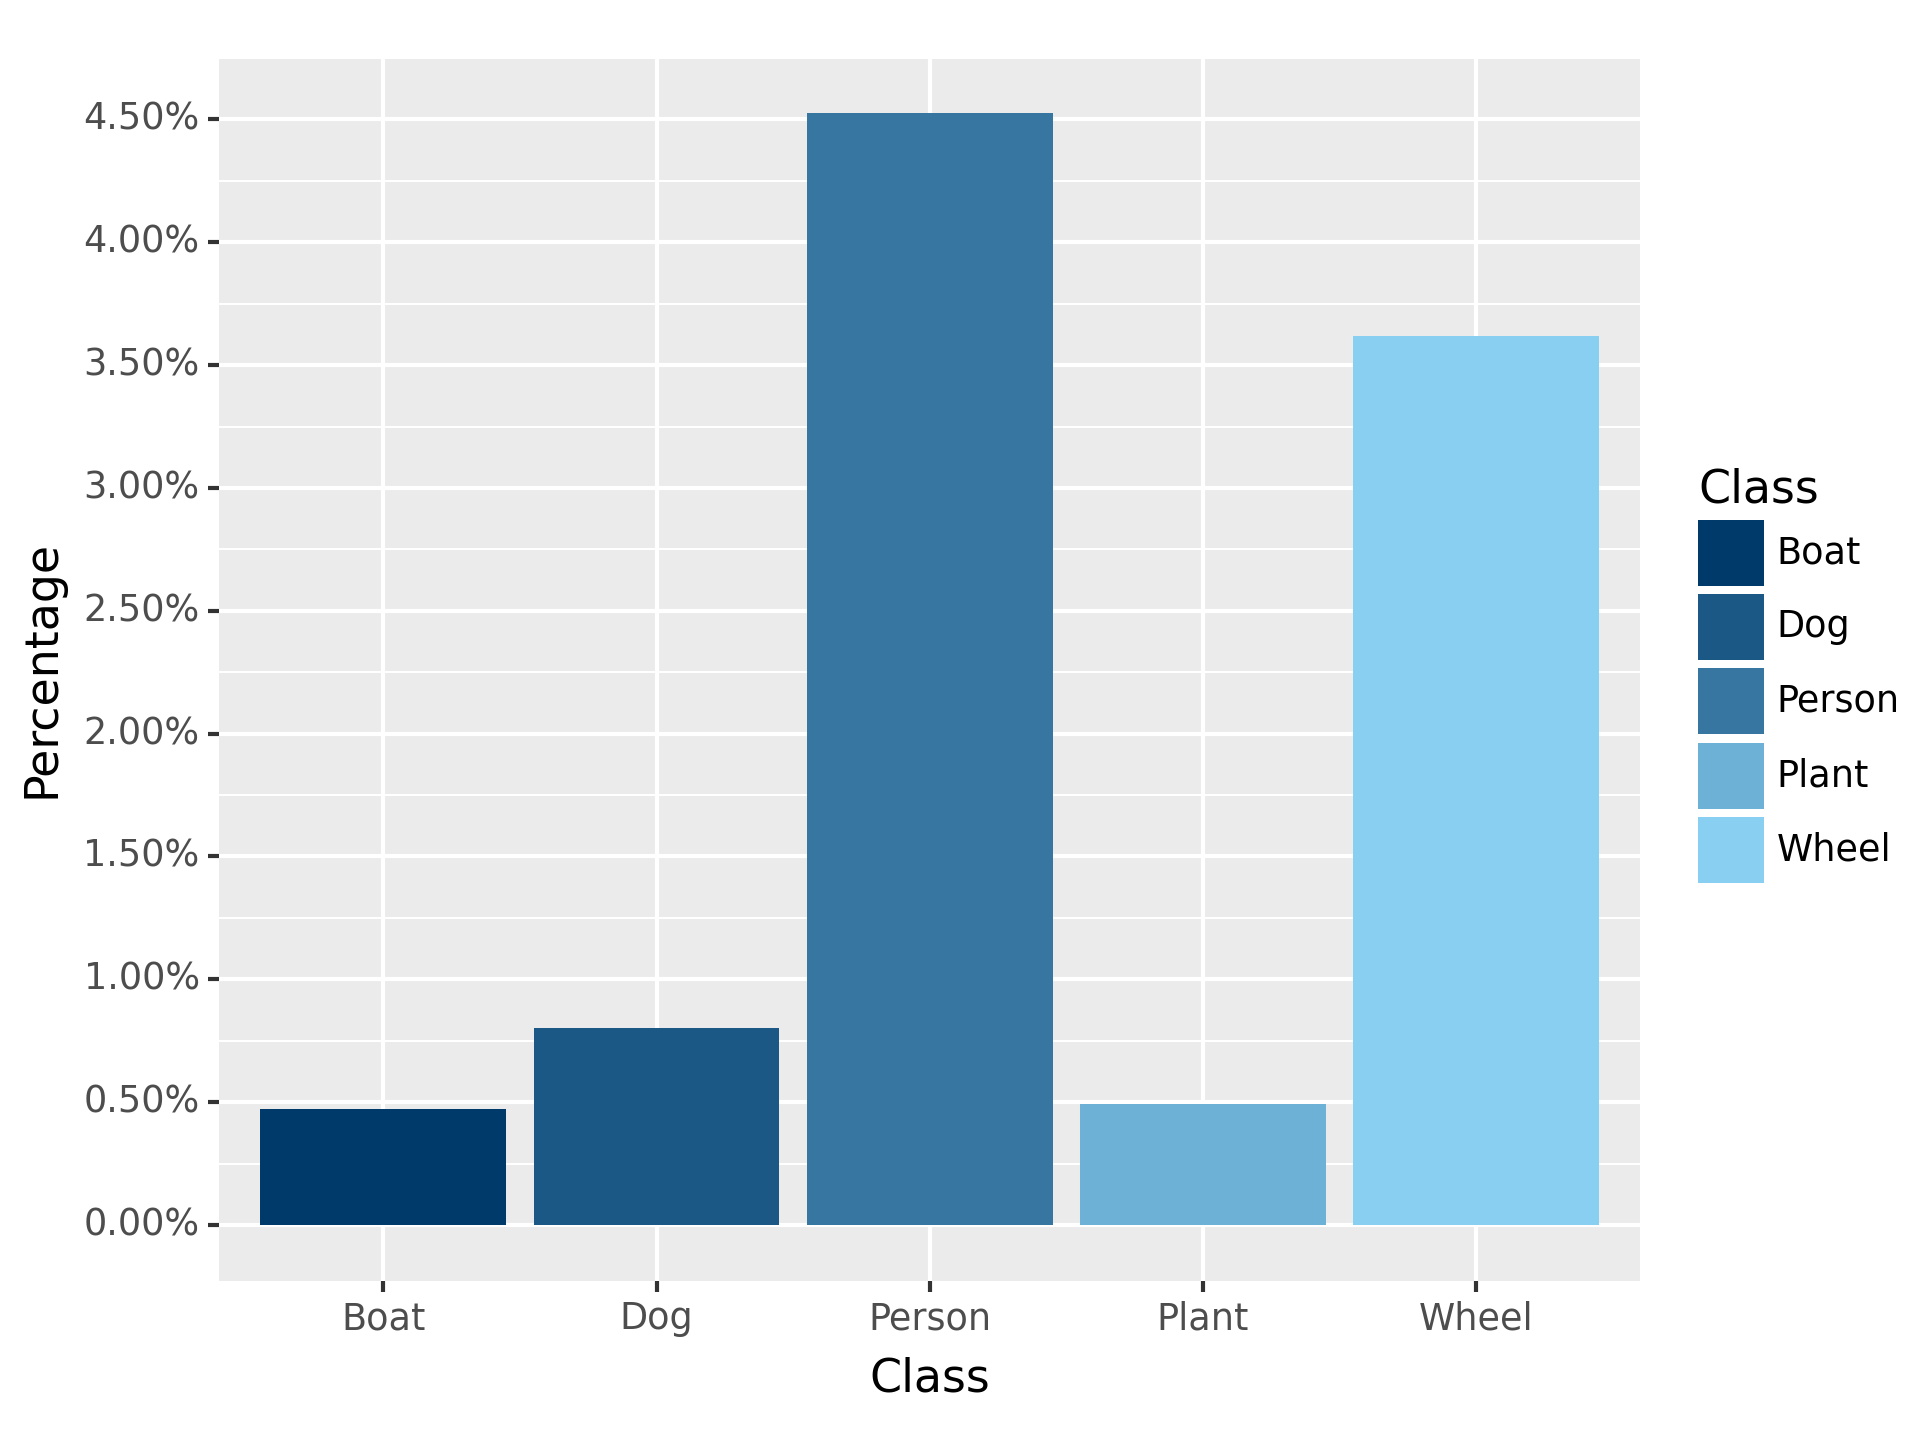
\includegraphics[width=0.70\textwidth]{../Data/distribution-classes-barchart.png}
  \caption{Class Usage in Dataset (\%)}
  \label{fig:class-usage-in-dataset}
\end{figure}
\\
Each snapshot was evaluated by using the above-mentioned images and the accuracy as well as the loss was saved in a CSV file for 
analysation.
\\
\subsection{Data Transformation and Visualisation}
Data transformation and its visualisation plays a crucial role in evaluating the hypothesis. The gathered data was exported to multiple CSV files, 
which were categorized by class and consisted of the number of iterations and the accuracy per picture. Python and Jupyter Notebooks were the
foundation for the handling of data in this project. Data manipulation was handled by Pandas and the visualisation was done using Matplotlib
and Plotnine.\\

% CLASS DISTRIBUTION
The annotations JSON file, included in the training dataset \parencite{pascal2023}, was an additional source of information. 
A custom Python script was written to transform the data into a useable format, which was required to calculate the class distribution 
and the image count per class. To illustrate which classes were evaluated and their representation in the dataset, a bar chart was created 
(See Fig.~\ref{fig:class-usage-in-dataset}). This choice was motivated by the observation that "[v]ertical bar charts are useful to compare 
different categorical [...] variables" \parencite{Statistics-Canada2021}.\\ 
\newpage

% LOSS GRAPH
The loss was graphed by using a scatter plot (See Fig.~\ref{fig:loss-vs-training-iterations})
as it visualises the relationship between two or more quantitative variables. They are especially helpful when examining whether
the values of one variable are influenced by the values of the other variable \parencite{Statistics-Canada2021b}. 
Additionally, a quadratic trend line was added to identify the trend and outliers.\\ 

% ACCURACY GRAPH
To plot the accuracy all CSV files were merged by iterating through each file, calculating the mean accuracy per iteration and appending it
to the new pandas data frame. This resulted in a data frame with the mean accuracy per iteration for each class. This data was then plotted using
a line chart (See Fig.~\ref{fig:accuracy-vs-training-iterations}). \\ 

% ACCURACY IMPROVEMENT GRAPH
To illustrate the improvement of accuracy over time, the average accuracy of all classes per iteration was calculated.
From that, the percentual increase of accuracy was calculated and then the average accuracy was plotted against the number of iterations
(See Fig.~\ref{fig:accuracy-improvement}).
A line chart was chosen for both because it is useful for illustrating trends over time \parencite{Statistics-Canada2021a}.\\

% BAR CHART FLUCTUATION WHEEL AND DOG
For further investigation into the performance of some classes, the accuracy for a specific iteration per picture was plotted 
using a line and bar chart (See Fig.~\ref{fig:14000-dog}, \ref{fig:image-1-accuracy}, \ref{fig:13000-wheel}, \ref{fig:image-3-accuracy}). 
This was done to identify outliers and to clearly display discrepancies in performance between pictures of the same class.\\

% BOX PLOT PER ITERATION
To obtain a comprehensive insight into the variation in the model's accuracies, a box plot was utilised (See. Fig~\ref{fig:Box-plot}). This visual representation illustrated the distribution of the accuracy measurements gathered during the experiment, portraying how the model evolved throughout its training process.
This graph is a good choice since its use case is illustrating the distribution of data \parencite{Tableau}.\\


\end{document}
	
	
\printbibliography[title=References]
	
	
	
	
	
	
	
	
	
	
	
	
	
	
	
	
	
	
	
	
	
	
\end{document}          
